\documentclass[a4paper, 12pt]{article}

\usepackage{cmap}
\usepackage{mathtext} 
\usepackage[T2A]{fontenc}
\usepackage[utf8]{inputenc}
\usepackage[english,russian]{babel}	

\usepackage{amsfonts,amssymb,amsthm,mathtools}
\usepackage{amsmath}
\usepackage{icomma} 

\usepackage{graphicx} 
\graphicspath{{Picturies/}}
\usepackage{wrapfig}

\usepackage{array,tabularx,tabulary,booktabs}
\usepackage{longtable}
\usepackage{multirow}

\usepackage{caption}
\captionsetup{labelsep=period}

\renewcommand{\phi}{\varphi}
\newcommand{\eps}{\varepsilon}
\newcommand{\parag}[1]{\paragraph*{#1:}}

\newcounter{Points}
\setcounter{Points}{1}
\newcommand{\point}{\arabic{Points}. \addtocounter{Points}{1}}

\author{Вязовцев Андрей, Б01-005}
\date{08.10.21}
\title{Лабораторная работа 3.3.5. Эффект Холла в металлах.}

\begin {document}

\maketitle

\parag {Цель работы} измерение подвижности и концентрации носителей заряда в металлах.

\parag {В работе используются} электромагнит с источником питания, источник постоянного тока, микровольтметр Ф116/1, амперметры, измеритель магнитной индукции Ш1-10, образцы из меди, серебра и цинка.

\parag {Теоретическая справка} ~\\

В магнитном поле $\vec{B}$ на заряды действует сила Лоренца:

\[
    \vec{F} = q\vec{E} + q\vec{u} \times \vec{B}
\]

В связи с этим направление движения зарядов может не совпадать с $\vec{E}$, поэтому их движение будет искривляться, или, если первое не позволяет геометрия проводника, будет возникать поперечное поле, противодействующее силе Лоренца. Возникновение этого поля называют эффектом Холла.

Закон Ома в дифференциальной форме записывается так:

\[
    \vec{j} = \sigma \vec{E} = \frac{\vec{E}}{\rho}
\]

Где $\sigma$ --- проводимость среды, $\rho$ --- удельное сопротивление, а $\vec{j}$ --- плотность тока, которая по определению равна:

\[
    \vec{j} = q n \vec{u}
\]

Здесь $n$ --- концентрация частиц, а $\vec{u}$ --- средний вектор скорости. Его можно выразить так:

\[
    \vec{u} = \mu \vec{E}
\]

Тогда зависимость проводимость от подвижности выражается так:

\[
    \sigma = q n \mu
\]

Для исследования зависимости проводимости используют две принципиально различные схемы: мостик Холла и диск Корбино. Рассмотрим первый, т.~к. на его основе будет проводиться лабораторная работа.

В этой схеме ток вынуждают течь по оси $x$ вдоль плоской пластинки (длиной $l$, толщиной $h$ и шириной $a$). Холловское напряжение в данном случае равно:

\[
    U_{\perp} = E_y a
\]

Где:

\[
    E_y = \rho_{yx} \cdot j_x = \frac{j_x B}{n q}
\]

Из выражения для полного тока $I$:

\[
    j_x = \frac{I}{a h}
\]

Получаем:

\[
    U_{\perp} = \frac{B}{n q h} \cdot I = R_H \cdot \frac{B}{h} \cdot I
\]

Где $R_H$ --- постоянная Холла:

\[
    R_H = \frac{1}{n q}
\]

\parag {Экспериментальная установка} ~

\begin{figure}[!h]
    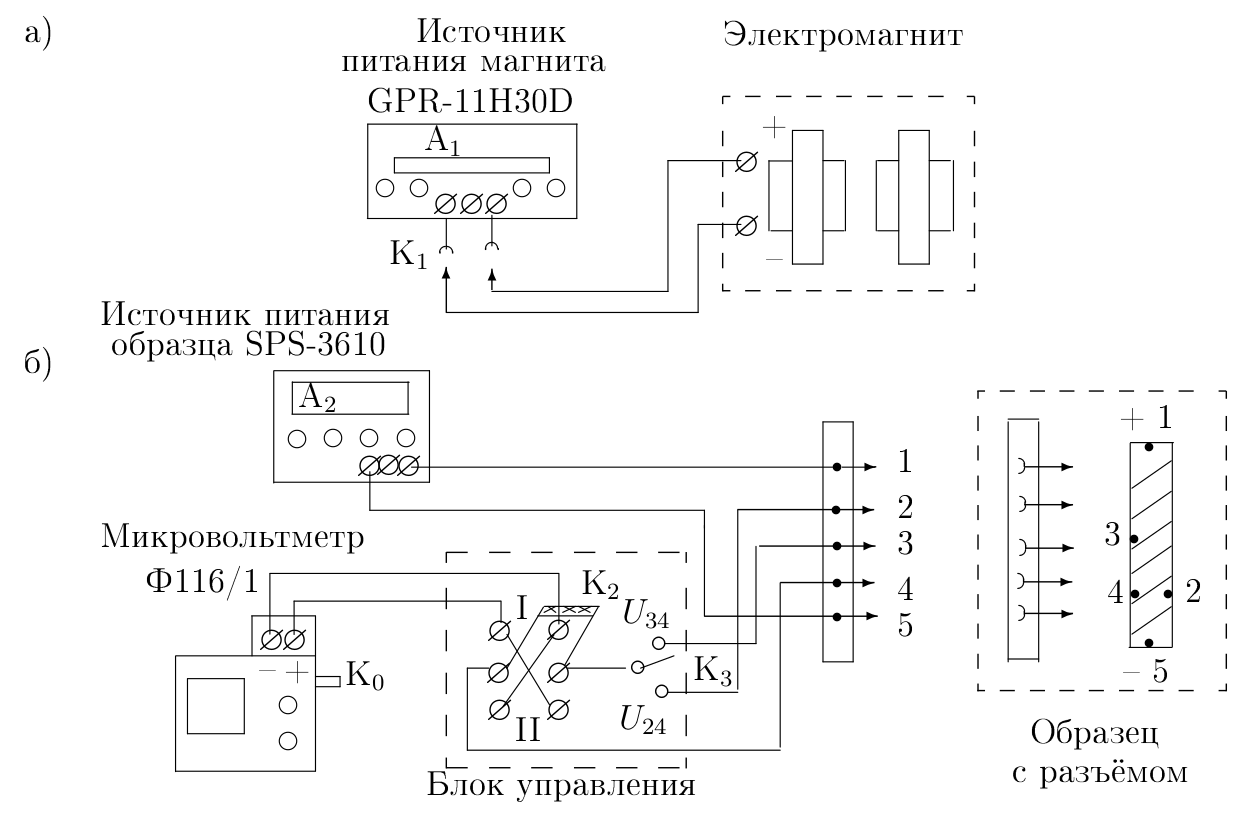
\includegraphics[scale = 0.2]{Workplace}
    \centering
    \caption{Схема установки для исследования эффекта Холла в металлах}
\end{figure}

В зазоре электромагнита создаётся постоянное магнитное поле, величину которого можно изменить с помощью регулятора тока источника. Градуировка магнита осуществляется с помощью измерителя магнитной индукции.

Металлические образцы в форме тонких пластинок подключаются к блоку питания через разъём.

\parag {Ход работы} ~\\

\point Настроим все измерительные приборы согласно методическим пособиям. 

\point Найдём максимальный ток через серебряный образец при напряжении $U_{пред-с} = 0,8$ В. Получаем: $I_{пред-с} = 1,1$ А.

\point Найдём предельное значение тока через электромагнит. Для этого сначала выведем напряжение на максимум ($U_{пред-м} = 2,6$ В), после чего --- ток. Получаем: $I_{пред-м} = 5,25$ А.

\point Найдём зависимость магнитной индукции $B$ от тока через магнит $I_M$, результаты занесём в таблицу:

\begin{table}[!h]
    \begin{tabular}{|c|c|c|c|c|c|c|c|c|} \hline
        $I_M$, А & 0.16 & 0.32 & 0.48 & 0.64 & 0.8 & 0.96 & 1.12 & 1.28 \\ \hline
        $B$, мТл & 204 & 347 & 575 & 752 & 911 & 1009 & 1078 & 1123 \\ \hline
    \end{tabular}
    \caption {Зависимость индукции электромагнита от тока через него}
\end{table}

\point Снимем зависимость напряжения $U = U_{24}$ (включая начальное напряжение $U_0$) от тока через магнит $I_M$ при фиксированном токе $I$ через образец. Проведём несколько серий измерений, изменяя $I$ и материал образца:

\begin{table}[!h]
    \begin{tabular}{|c|c|c|c|c|c|c|c|c|}
        \hline
        I, А & 0.16 & 0.32 & 0.48 & 0.64 & 0.8 & 0.96 & 1.12 & 1.28\\ \hline
        U, нВ & 240 & 280 & 400 & 480 & 600 & 640 & 680 & 760 \\ \hline
    \end{tabular}
    \caption {Зависимость $U (I_M)$ для серебряного образца при $I = 0,6$ А}
\end{table}

\begin{table}[!h]
    \begin{tabular}{|c|c|c|c|c|c|c|c|c|}
        \hline
        I, А & 0.16 & 0.32 & 0.48 & 0.64 & 0.8 & 0.96 & 1.12 & 1.28\\ \hline
        U, нВ & 240 & 360 & 600 & 720 & 880 & 920 & 1000 & 1040 \\ \hline
    \end{tabular}
    \caption {Зависимость $U (I_M)$ для серебряного образца при $I = 0,9$ А}
\end{table}

\begin{table}[!h]
    \begin{tabular}{|c|c|c|c|c|c|c|c|c|}
        \hline
        I, А & 0.16 & 0.32 & 0.48 & 0.64 & 0.8 & 0.96 & 1.12 & 1.28\\ \hline
        U, нВ & 320 & 560 & 760 & 920 & 1120 & 1200 & 1280 & 1320 \\ \hline
    \end{tabular}
    \caption {Зависимость $U (I_M)$ для серебряного образца при $I = 1,2$ А}
\end{table}

\begin{table}[!h]
    \begin{tabular}{|c|c|c|c|c|c|c|c|c|c|}
        \hline
        I, А & 0 & 0.16 & 0.32 & 0.48 & 0.64 & 0.8 & 0.96 & 1.12 & 1.28 \\ \hline
        U, нВ & 480 & 760 & 1040 & 1240 & 1520 & 1720 & 1800 & 1880 & 1920 \\ \hline
    \end{tabular}
    \caption {Зависимость $U (I_M)$ для цинкового образца при $I = 1,0$ А}
\end{table}

\point Определим, каким типом проводимости обладает каждый материал. Получаем: в серебряном образце носителями являются электроны, а у цинка - дырки. Из этого следует, что постоянная Холла $R_H$ для цинка будет положительна, а для серебра --- отрицательна.

\point Выключим источник питания электромагнита и установим переключатель микровольтметра в положение $750$ мкВ. Теперь при $I = 1$ А измерим падение напряжение между контактами 3 и 4 для каждого из двух образцов. Получаем: $U_{цинка} = 48$ мкВ, $U_{серебра} = 38$ мкВ.

\point Запомним характеристики пластин.

Цинк: $L_{3,4} = 3,5$ мм, $l = 9$ мм, $h = 0,12$ мм.

Серебро: $L_{3,4} = 15$ мм, $l = 11$ мм, $h = 0,09$ мм.

\point Построим график зависимости $B = f (I_M)$

\point Построим графики зависимостей $\eps = f(B)$ при различных значениях тока для цинка и меди. Определим коэффициенты наклона прямых: 

\begin{align*}
    K_{1-Ag} (I) = (0,55 \pm 0,02) \cdot 10^{-6}~\frac{В}{Тл}\\
    K_{2-Ag} (I) = (0,86 \pm 0,02) \cdot 10^{-6}~\frac{В}{Тл} \\
    K_{3-Ag} (I) = (1,05 \pm 0,03) \cdot 10^{-6}~\frac{В}{Тл} \\
    K_{Zn} (I) = (1,28 \pm 0,04) \cdot 10^{-6}~\frac{В}{Тл}
\end{align*}

\point Найдём постоянную Холла для всех экспериментов, учтём тот знак, который был определён выше. Воспользовавшись соотношением:

\[
    K (I) = \frac{R_H \cdot I}{h}
\]

Получаем:

\begin{align*}
    R_{H1-Ag} = - (8,3 \pm 0,2) \cdot 10^{-11} \frac{м^3}{Кл} \\
    R_{H2-Ag} = - (8,6 \pm 0,2) \cdot 10^{-11} \frac{м^3}{Кл} \\
    R_{H3-Ag} = - (7,9 \pm 0,2) \cdot 10^{-11} \frac{м^3}{Кл} \\
    R_{H-Zn} =  + (1,5 \pm 0,1) \cdot 10^{-10} \frac{м^3}{Кл}
\end{align*}

\point Теперь найдём концентрацию $n$ носителей тока. При этом коэффициент Холла серебра возьмём как среднее арифметическое результатов 1-3. Воспользуемся формулой:

\[
    n = \frac{1}{R_H q}
\]

Получаем:

\begin{align*}
    n_{Ag} = (7,5 \pm 0,2) \cdot 10^{28} ~м^{-3} \\
    n_{Zn} = (4,2 \pm 0,2) \cdot 10^{28} ~м^{-3}
\end{align*}

\point Найдём удельную проводимость материалов:

\begin{align*}
    \sigma_{Ag} = (39,9 \pm 0,8) \cdot 10^6 ~\frac{1}{Ом \cdot м}
    \sigma_{Zn} = (6,7 \pm 0,4) \cdot 10^6 ~\frac{1}{Ом \cdot м}
\end{align*}

\point Найдём подвижность носителей тока:

\begin{align*}
    \mu_{Ag} = 33,1 \pm 0,7 ~\frac{см^2}{В \cdot с}
    \mu_{Zn} = 10,1 \pm 0,4 ~\frac{см^2}{В \cdot с}
\end{align*}

\parag{Вывод} ~\\

Табличные значения таковы: $R_{H-Ag} = - 9 \cdot 10^{-11}$, $R_{H-Zn} = + 5,5 \cdot 10^{-11}$. Таким образом, значение для серебра практически совпало, а для цинка отличается в три раза. Скорее всего, это связано с примесями в металле.

\begin{figure}[!h]
    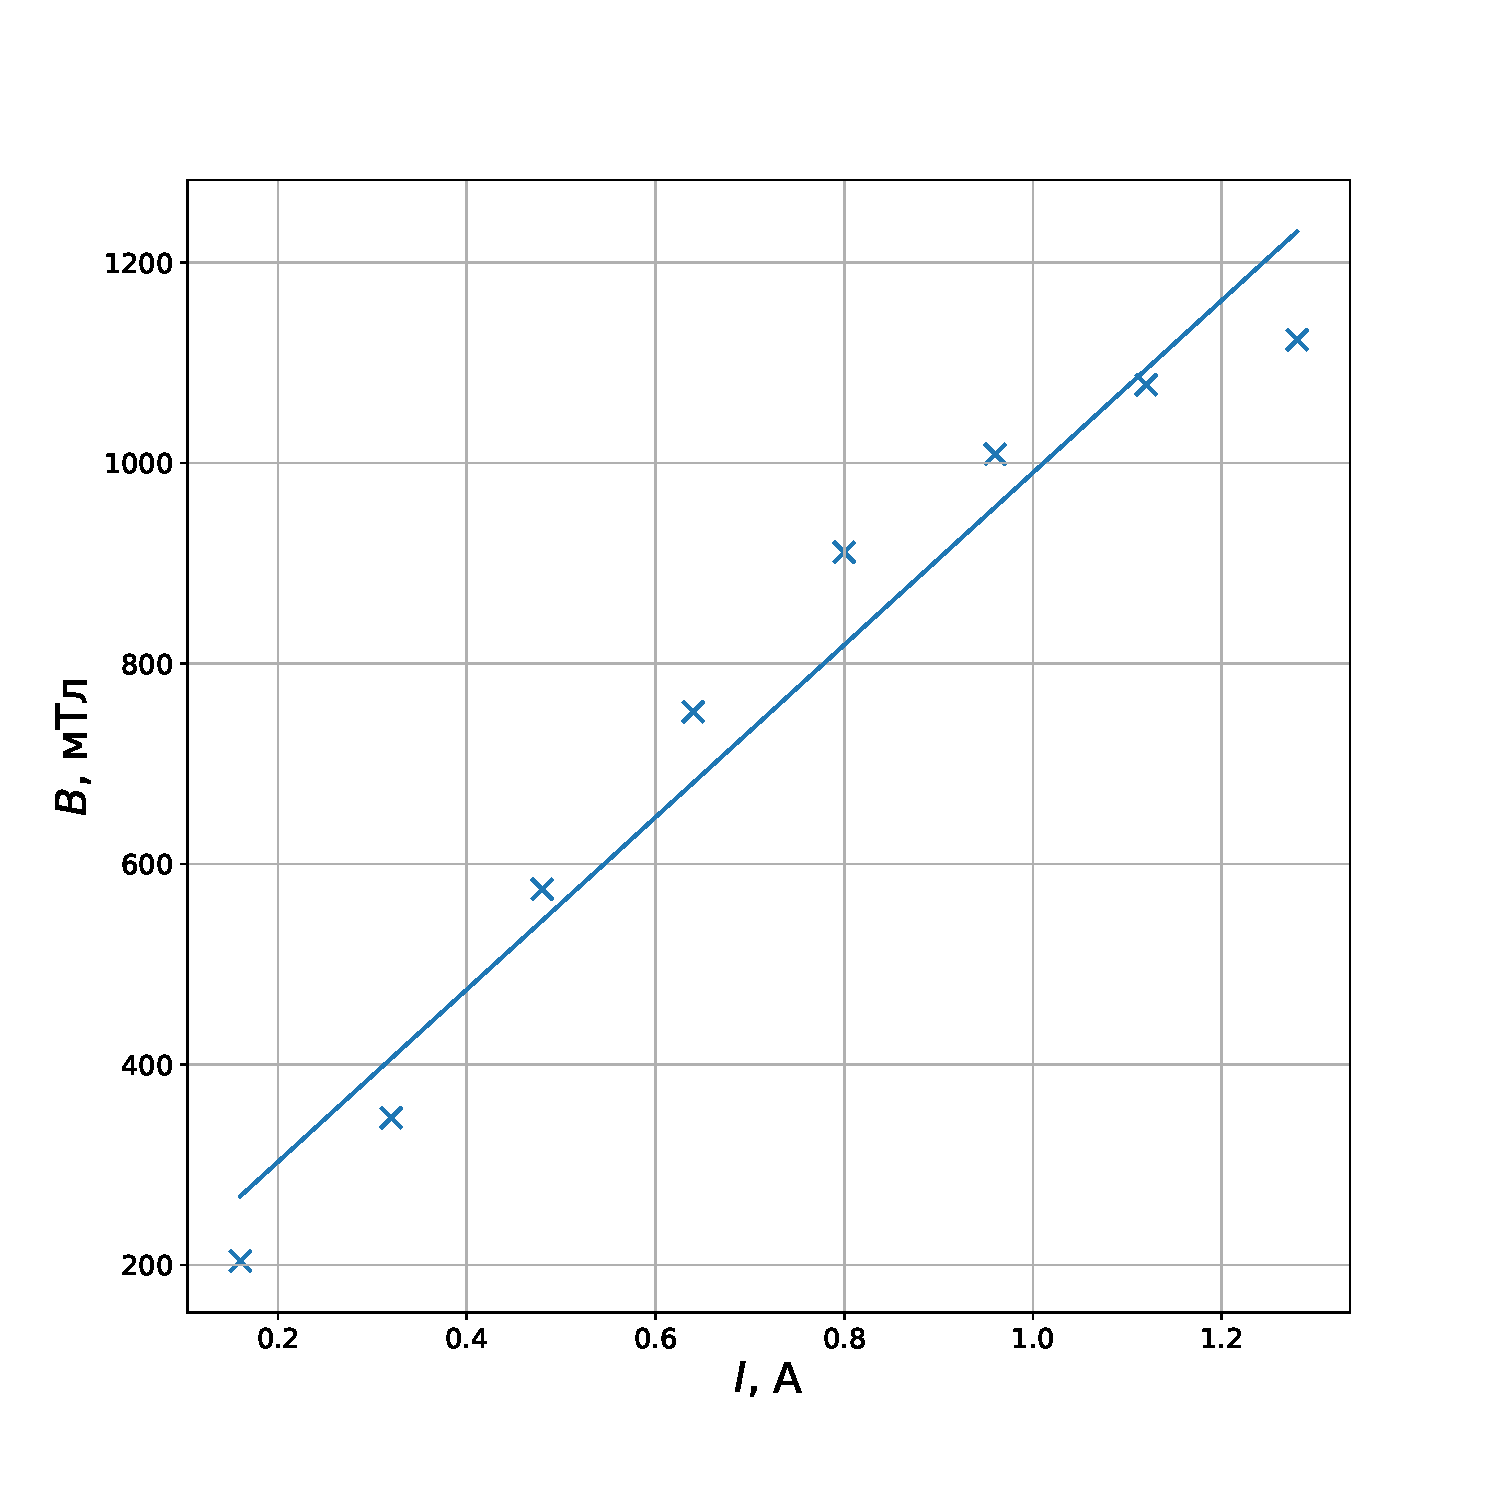
\includegraphics[scale = 0.35]{B_I}
    \centering
    \caption{График $B (I)$}
\end{figure}

\begin{figure}[!h]
    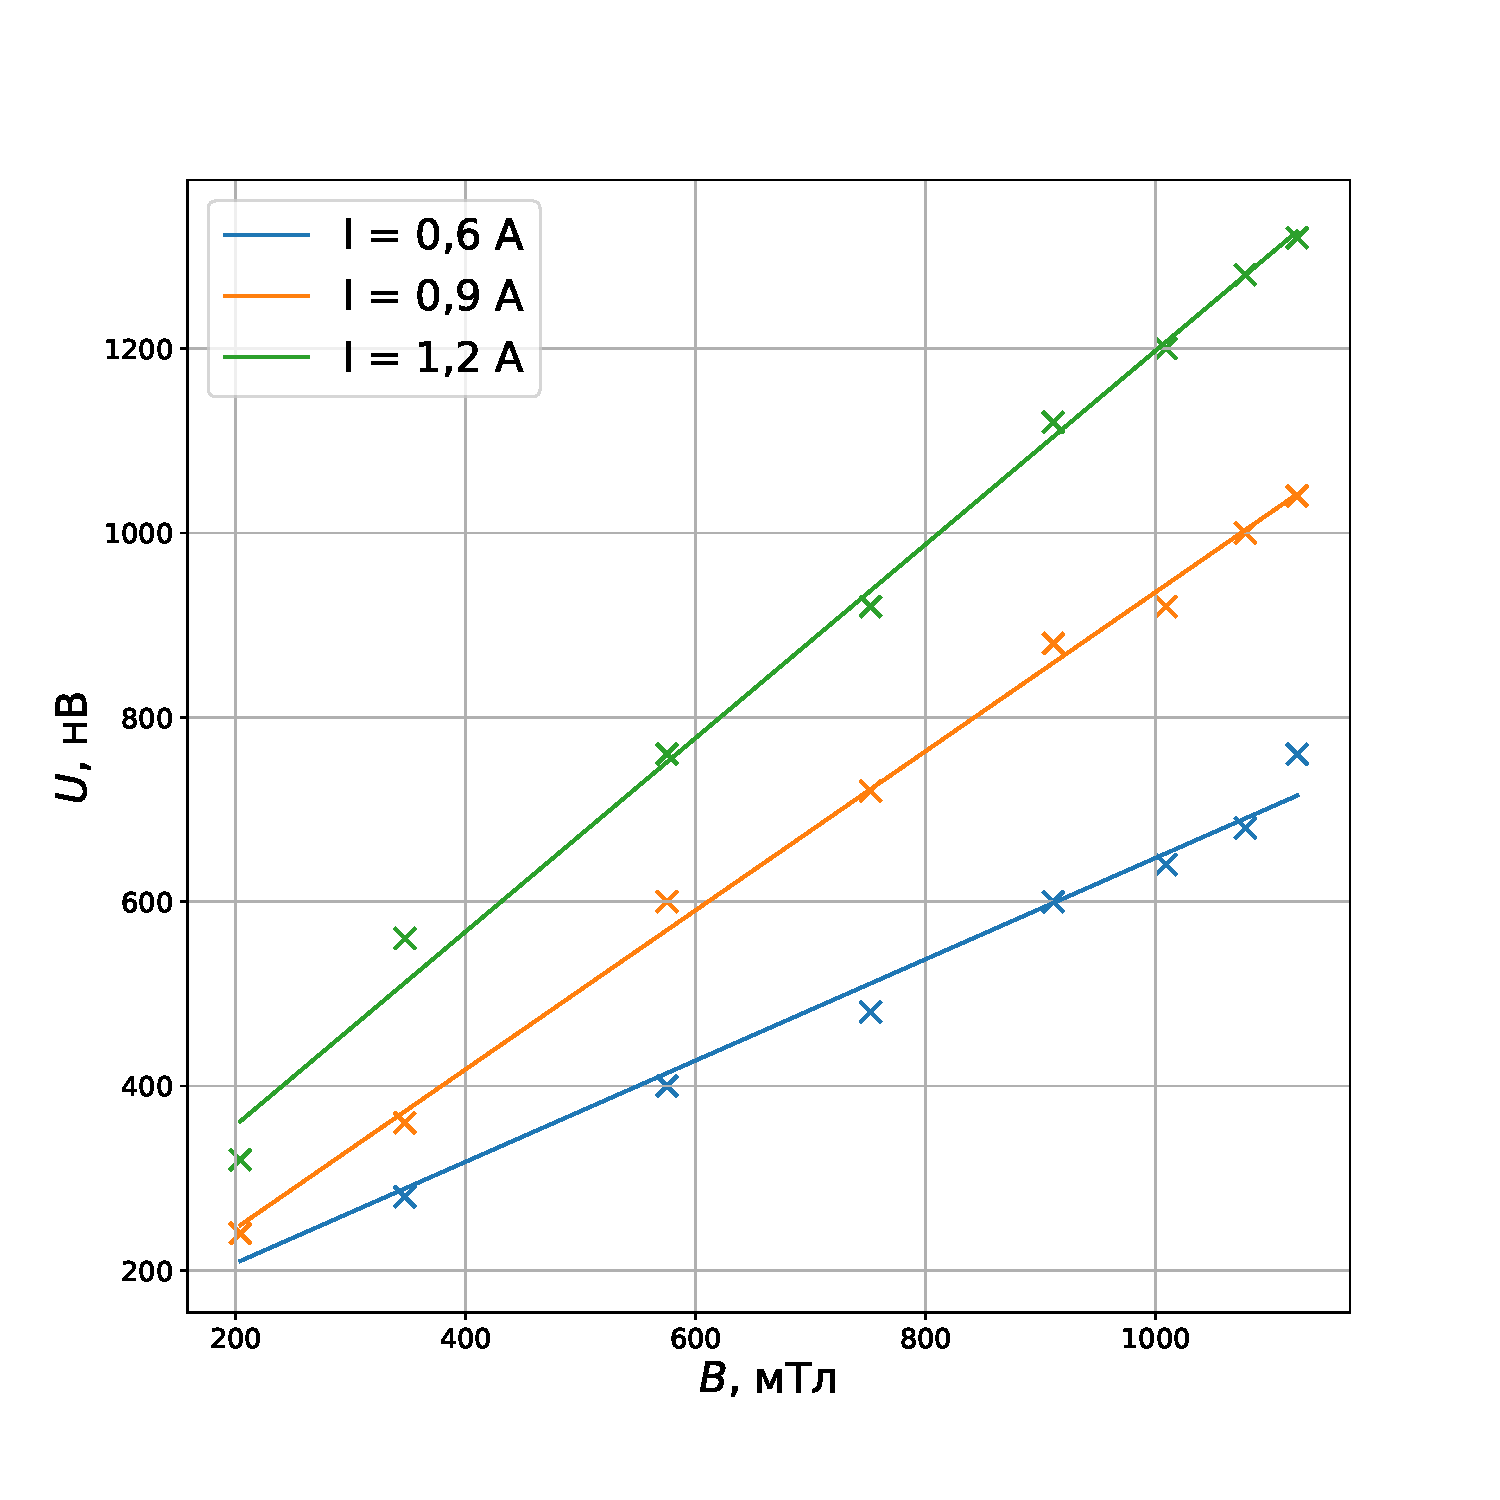
\includegraphics[scale = 0.35]{Silver}
    \centering
    \caption{График $\eps (B)$}
\end{figure}

\begin{figure}[!h]
    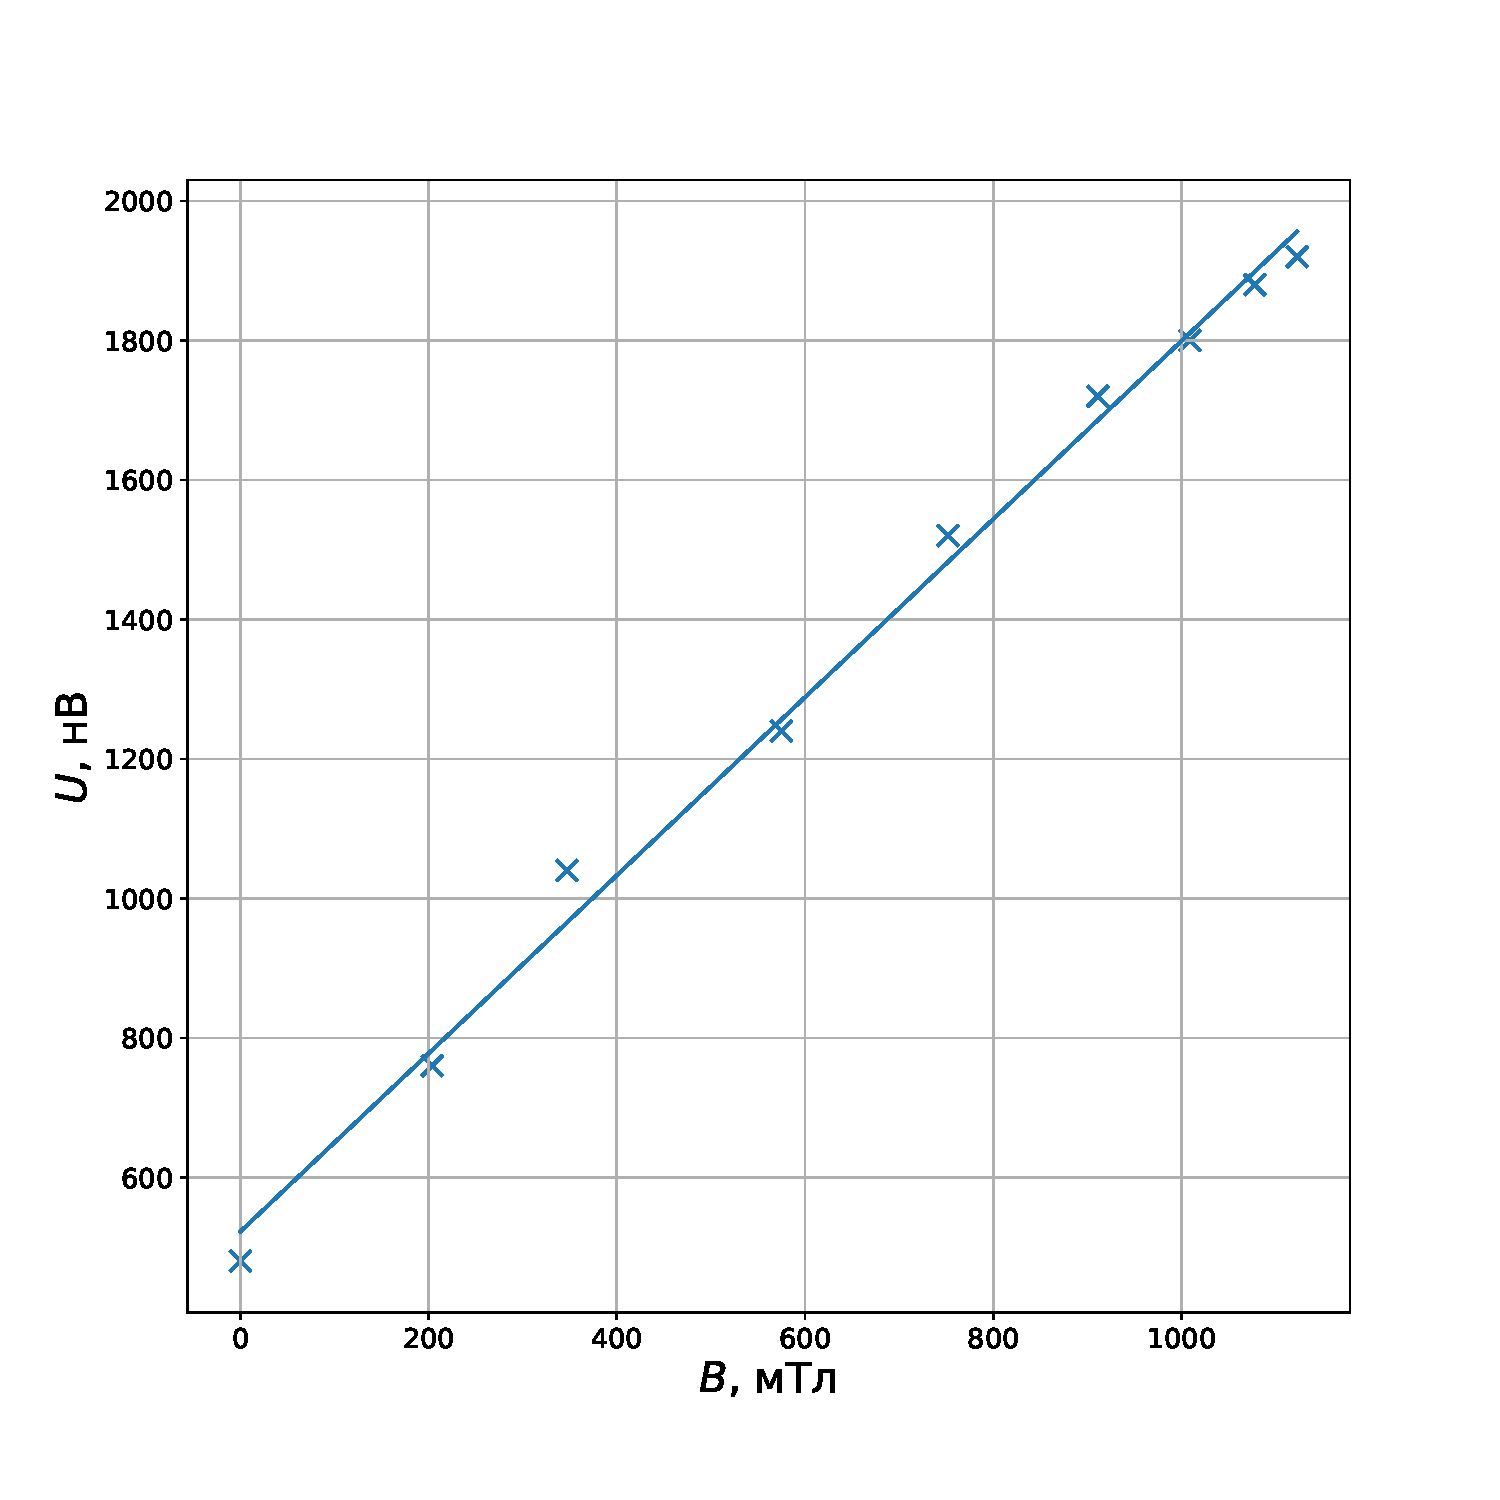
\includegraphics[scale = 0.35]{Zinc}
    \centering
    \caption{График $\eps (B)$}
\end{figure}

\end {document}
